\documentclass[bluish,slideColor,colorBG,pdf]{prosper}
\hypersetup{pdfpagemode=FullScreen}
\usepackage{graphicx}
\usepackage{epsfig}
\def\baselinestretch{1.0}
\setlength{\topmargin}{-60pt}
\setlength{\textheight}{460pt}
\setlength{\oddsidemargin}{0pt}
\setlength{\evensidemargin}{0pt}
\setlength{\textwidth}{660pt}
\setlength{\footskip}{0pt}
\parindent 0.3in
\hyphenpenalty=10000
\tolerance=10000
\pagestyle{empty}

\def\Prob{{\rm Prob\;}}
\def\prob{{\rm \;Prob\;}}


\author{February 2017}
\title{Genome 562}
\institution{Week 5}

\begin{document}

\maketitle

\begin{slide}[Replace]{Approach to mutational equilibrium}

\centerline{\includegraphics[height=2.5in]{fig3-1.idraw}}

\end{slide}

\begin{slide}[Replace]{Mutation vs. selection: effect of dominance}

\centerline{\includegraphics[height=2.5in]{fig3-2.idraw}}

\end{slide}

\begin{slide}[Replace]{Mutational load: effect of dominance}

\centerline{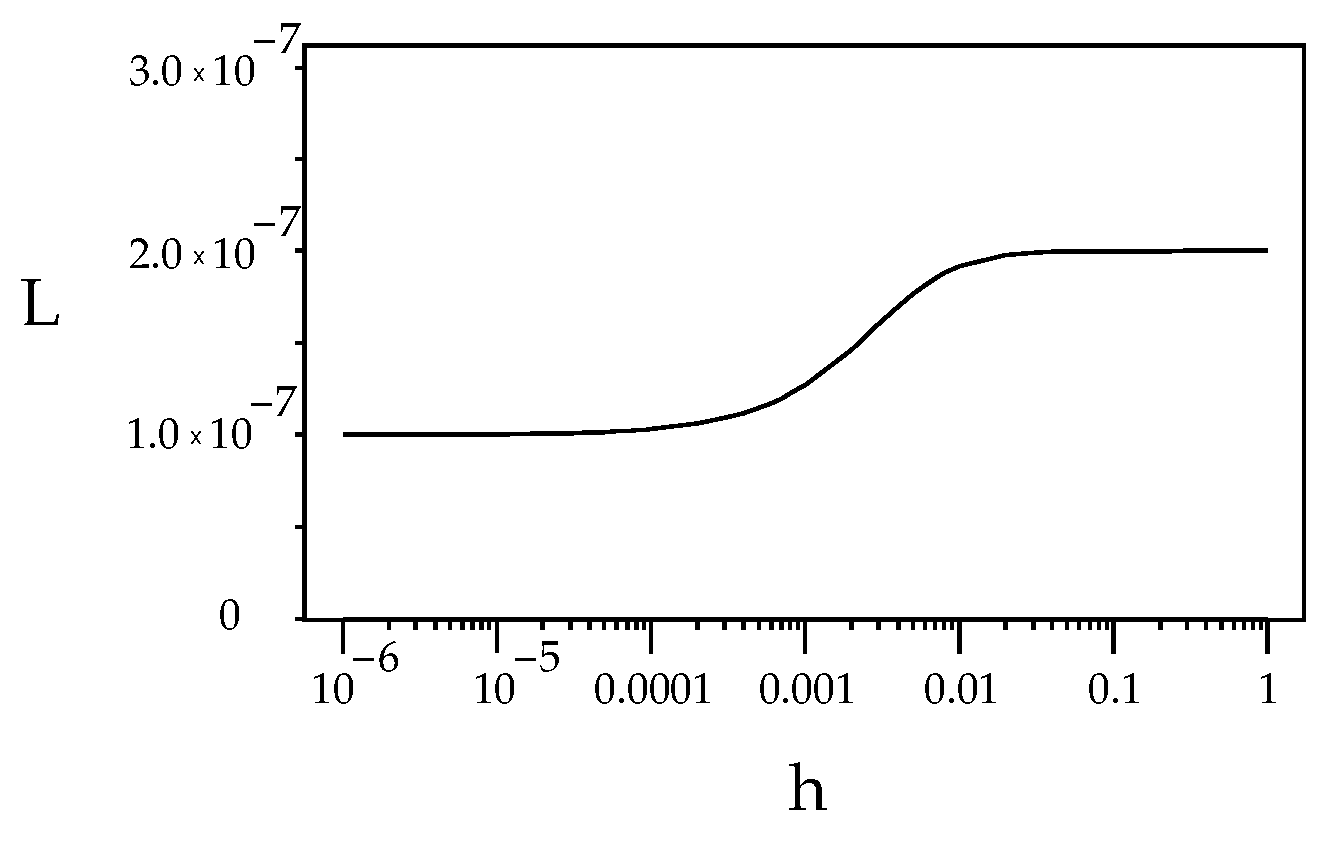
\includegraphics[height=2.5in]{fig3-3.ps}}

\end{slide}

\begin{slide}[Replace]{Hermann Joseph Muller (1890-1967) }

\begin{center}
\begin{tabular}{c c}
\includegraphics[height=2in]{Muller1945ish.ps}\\
& \\
in about 1945 \\
\end{tabular}
\end{center}
\bigskip

The greatest classical geneticist. Nobel Prize in 1945. Proved by elegant
chromosome manipulations that radiation could induce mutations.

\end{slide}

\begin{slide}[Replace]{Has ``junk DNA'' been a delusion? }
\vspace{-0.08in}

{\tiny
The 2012 papers by the ENCODE project reported that ``These data enabled us to assign biochemical functions for 80\% of the genome,
in particular outside of the well-studied protein-coding regions.''

Popular science news media ran with the dramatic story (summary from T. Ryan
Gregory's ``Genomicron'' blog):
\vspace{-0.05in}
\hspace{-0.20in} \begin{itemize}
\addtolength{\itemsep}{-0.5\baselineskip}
\item New York Times -- Bits of Mystery DNA, Far From `Junk', Play Crucial Role
\item Los Angeles Times -- ENCODE project sheds light on human DNA and disease
\item Washington Post --  `Junk DNA' concept debunked by new analysis of human genome
\item Wall Street Journal -- `Junk DNA' Debunked
\item USA Today -- Researchers: `Junk' DNA plays major role in disease
\item NPR -- Scientists Unveil `Google Maps' For Human Genome
\item CNN -- DNA project interprets `book of life'
\item Scientific American -- Hidden Treasures in `Junk' DNA
\item MSNBC -- New DNA project shows us living beyond our genes
\item The Guardian (UK) -- Breakthrough study overturns theory of `junk DNA' in genome
\item The Independent (UK) -- Scientists debunk `junk DNA' theory to reveal
vast\\
\vspace{-2pt}
majority of human genes perform a vital function
\item The Telegraph (UK) -- Worldwide army of scientists cracks the `junk DNA' code
\item The Economist (UK) -- The new world of DNA
\item New Scientist (UK) -- Global project reveals just how active our `junk' DNA is
\item BBC (UK) -- Detailed map of genome function
\item The Globe and Mail (Canada) -- Worldwide group of scientists solve `junk
DNA'\\
\vspace{-2pt} mystery
\end{itemize}
}

But is it true?

\end{slide}

\begin{slide}[Replace]{One-island model}

\centerline{\includegraphics[height=2in]{fig4-1.ps}}

\end{slide}

\begin{slide}[Replace]{Island model}

\centerline{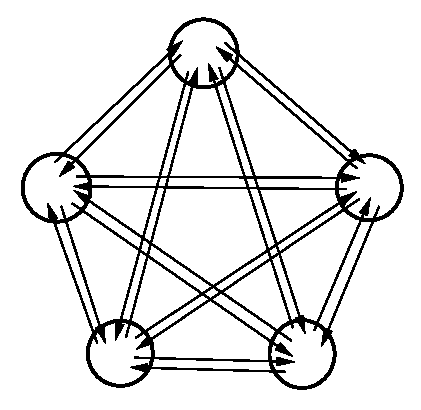
\includegraphics[height=2in]{fig4-2.ps}}

\end{slide}

\begin{slide}[Replace]{Collapse of a patch of adaptation}

\centerline{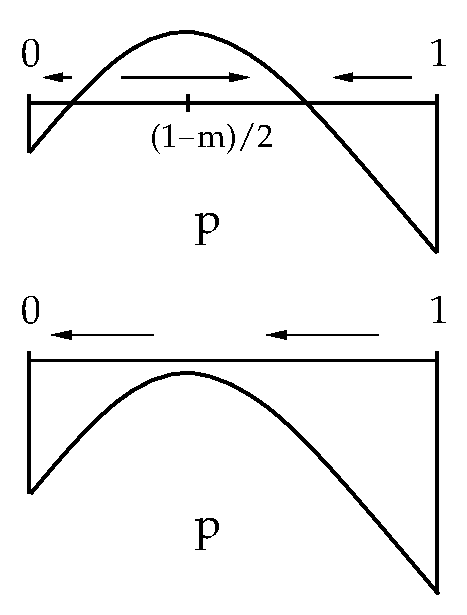
\includegraphics[height=2.5in]{fig4-3a.ps}}

\end{slide}

\begin{slide}[Replace]{Stepping-stone models}

\centerline{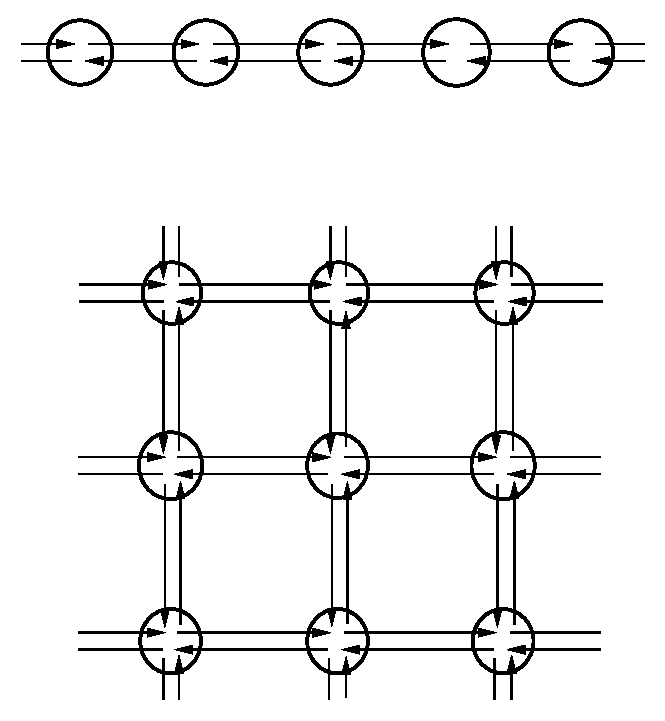
\includegraphics[height=2.5in]{fig4-3.ps}}

\end{slide}

\begin{slide}[Replace]{Selection versus migration: two populations}

\centerline{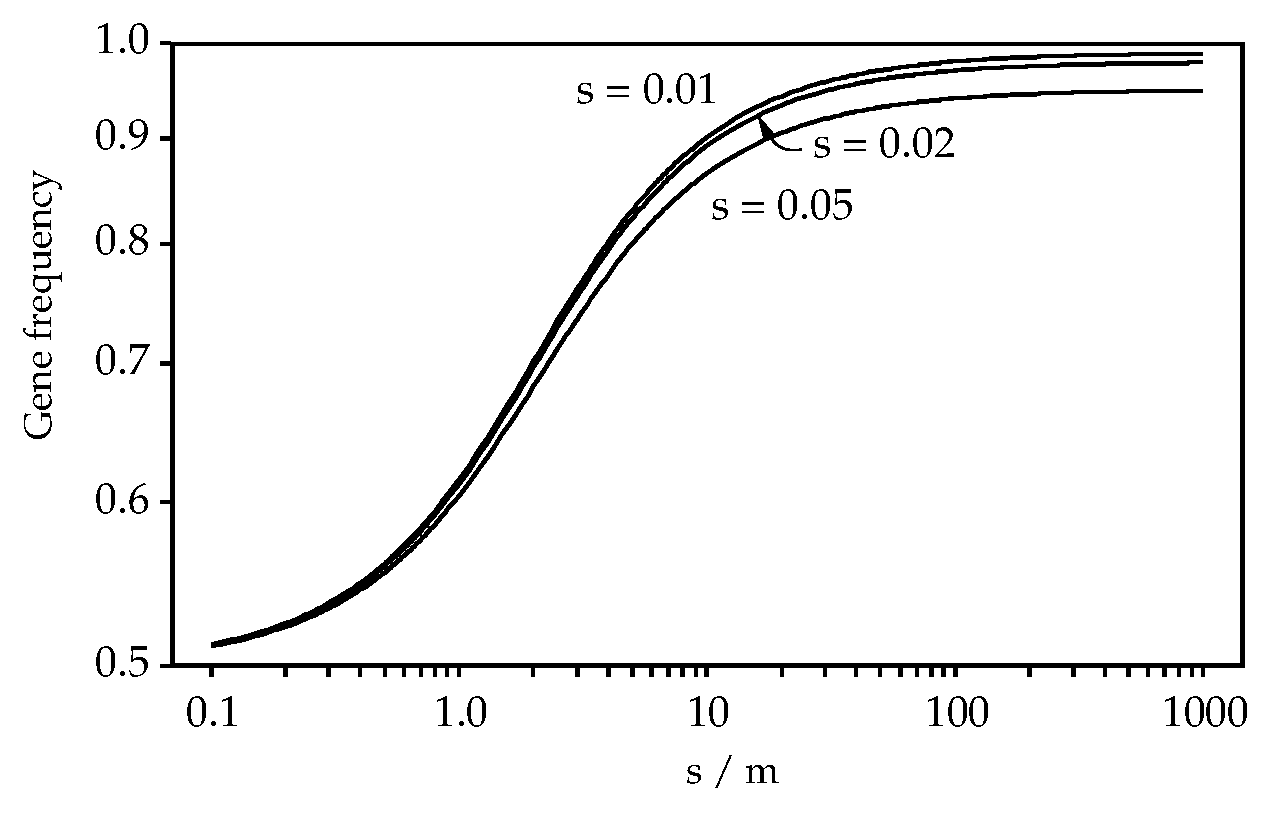
\includegraphics[height=2.5in]{fig4-4.ps}}

\end{slide}

\begin{slide}[Replace]{Clines}

\centerline{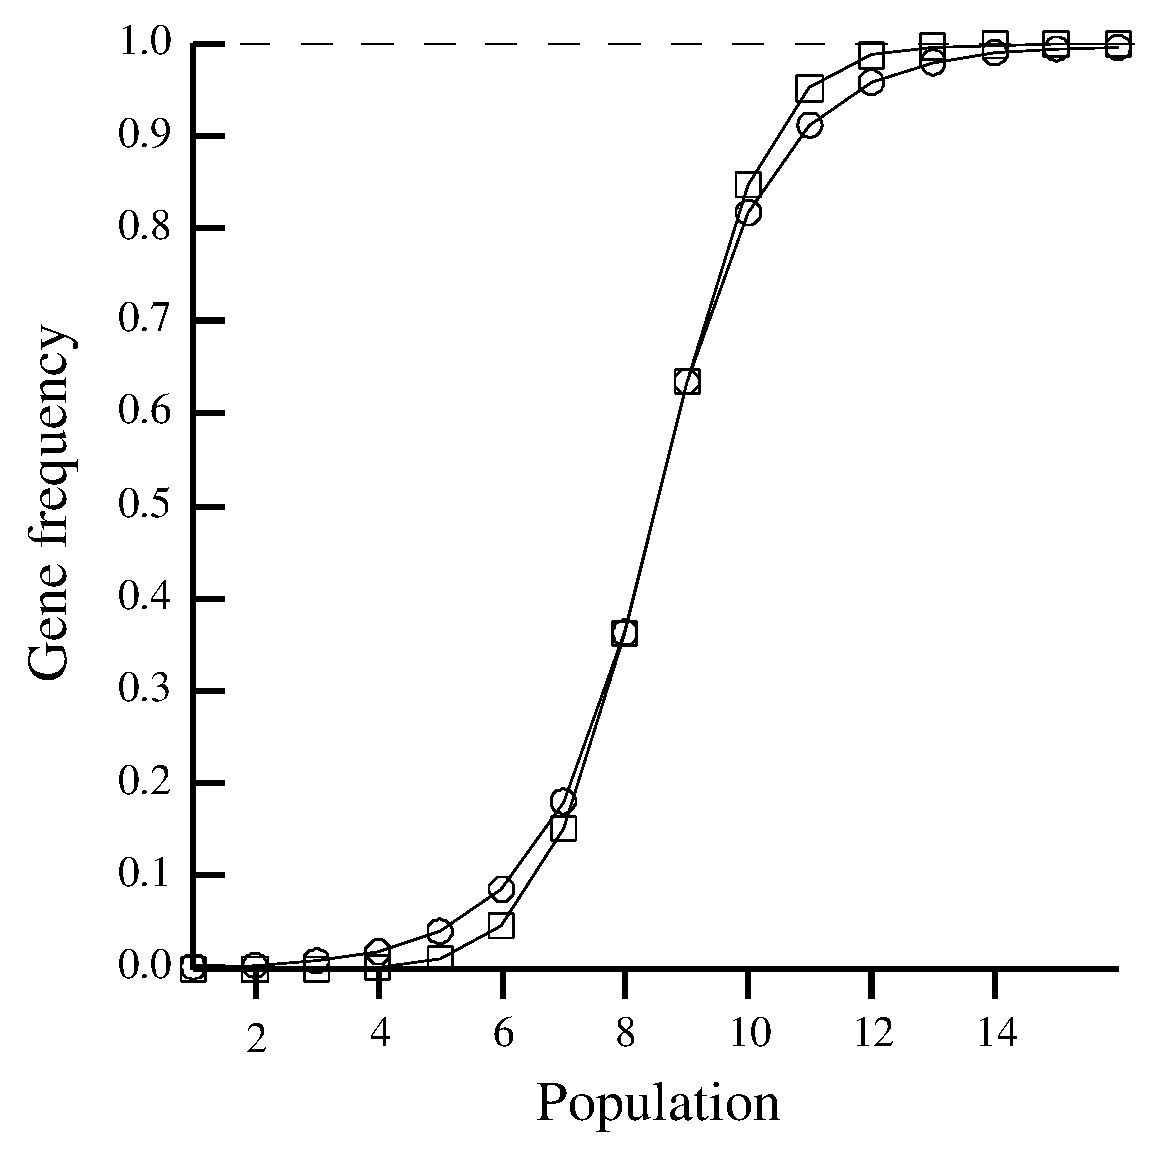
\includegraphics[height=3.0in]{fig4-5.ps}}

\end{slide}

\end{document}
